\documentclass[11pt]{article}

\usepackage{listings}
\usepackage{graphicx}

\begin{document}
\title{%
  N Queens \\
  \large A distributed approach to the N Queens algorithm}
\author{Jarred Parr}
\date{November 2018}
\maketitle

\section{Introduction}
The N Queens algorithm is a problem in which the outcome is the number of unique ways n queens can be placed on an n by n
chess board. The difficulty of this algorithm lies in the number of unique ways that this system can be presented. Due to the fact
that there are a number of ways it can be solved, but also that there is not a naive approach that expands easily to greater sizes of n. Because of this, additional care needs to be considered to achieve a reasonable runtime for an expanding value ofn.

\section{Program Architecture}
Per the specification, there only needed to be an algorithm that could produce a total number of solutions to the problem given some nonzero value n. There were a few approaches I attempted, but the main one was focused largely around the use of a depth first search algorithm to speed up the backtracking process. Each version is outlined as follows:

\subsection{Naive Backtracking}
The naive backtracking approach is a decently quick approach to solving the problem. Utilizing the recusrive element and memoization we are able to store the state consistently to prevent recalculation. However since a lot of array operations were being performed, it was not quite as fast as it could have possibly been.
This code was naive in that it also didn't account for cases where checks weren't necessary like in the case of very early in the large board or at the very end where checking all possible outcomes would not be needed.

\lstset{frame=tb,language=c++}
\begin{lstlisting}
 /**
 * Sequential runs until all n queens
 * have been placed
 */
auto sequential() {
  if constexpr (n == 0) {
    return false;
  }
  // Start with 2d vector of zeros with game board dims
  std::vector<std::vector<int>> game_board(n, std::vector<int>(n, 0));
  if (!sequential_helper(game_board, 0)) {
    std::cout << "No solutions." << std::endl;
    return EXIT_SUCCESS;
  }

  print(game_board);
  return EXIT_SUCCESS;
}

bool valid_spot(
  const std::vector<std::vector<int>>& game_board,
  int row,
  int col
) const {
  for (int i = 0; i < col; ++i) {
    if (game_board[row][i])
      return false;

    for (int i = row, j = col; i >= 0 && j >=0; --i, --j) {
      if (game_board[i][j])
        return false;
    }

    for (int i = row, j = col; j >= 0 && i < n; ++i, --j) {
      if (game_board[i][j])
        return false;
    }
  }
  return true;
}

bool sequential_helper(
  std::vector<std::vector<int>>& game_board,
  int col
) {
  if (col >= n) {
    return true;
  }

  for (int i = 0; i < n; ++i) {
    if (valid_spot(game_board, i, col)) {
      game_board[i][col] = 1;

      // Recurse!
      if (sequential_helper(game_board, col + 1))
        return true;

      // Backtrack if this doesn't work
      game_board[i][col] = 0;
    }
  }

  return false;
}
\end{lstlisting}
As can be seen, the code snippet was almost 60 lines and spanned 3 different functions each with their own goals. This was good enough as a start but it left something more to be desired in terms of structure and eventual performance as it was found in the distributed case to not do quite as well as the depth-first approach, which was not extremely optimized either, but it was a welcome improvement.

\subsection{Depth-First Backtracking Approach}
The Depth-First Backtracking approach was a nice marrying of previous ideas and newfound approaches after reading about the problem in online forums. It combined the speed and
elegance of the recurisve solution with the more straightforward and shortened approach found in the graph based solutions to similar problems.
Depth first search involves delving as deep as one can get down a particular path until no more can be explored, then going down each suboroute until we end back where we started which, in this case, is the first part of our game board (the \"backtrack\" part of the backtracking algorithm).
This approach was not only about 23\% faster, but was also about 20 lines of code shorter as it only needed two functions instead of 3.
\lstset{frame=tb,language=c++}
\begin{lstlisting}
auto sequential() {
  std::vector<std::vector<std::string>> valid;
  std::vector<int> queens;
  sequential_helper(valid, queens);

  return valid.size();
}

void sequential_helper(
  std::vector<std::vector<std::string>>& done,
  std::vector<int>& queens
) {
  if (queens.size() == n) {
    done.emplace_back();
    for (auto i = 0u; i < n; ++i) {
      done.back().emplace_back(n, '.');
      done.back().back()[queens[i]] = 'Q';
    }
  } else {
    for (auto i = 0u; i < n; ++i) {
      bool valid = true;

      for (auto j = 0u; valid && j < queens.size(); ++j) {
        valid = (queens[j] != i) &&
          (abs(queens[j] - i) != queens.size() - j);
      }

      if (valid) {
        queens.push_back(i);
        sequential_helper(done, queens);
        queens.pop_back();
      }
    }
  }
}
\end{lstlisting}
This more focused approach dealt with only performing some operations when they were explicitly necessary. It left out cases where extra searching was not needed and terminated the loop early if a collisison was detected instead of linearly scanning the rows and columns of the game board every time.

\section{Parallel Computation of N Queens}
This section of the assignment brought about the most difficulty. As a first time user of the MPI platform I seemed to struggle with nearly every possible problem. Not to mention
the infrastructure being in and out at times made accurate results difficult to use and benchmark things reliably. Random node failure was also a common occurance when this problem began to enter the 16$\times$16+ game board sizes. The results that were calculated showed < 1 speedup for the very small examples, but it was clear that the distributed system was able to shine significantly more when larger problems were thrown at it.
My two parallel solutions are as follows:

\subsection{The Naive Approach}
The naive approach adapts the $pi.cc$ code that was provided by Dr\. Wolffe to work as a proof of concept. This offered very minimal speedup but gave a good indication of how
the compilation process would work as well as the systems in place which allowed for code to be distributed across multiple notes. This can be seen below:
\lstset{frame=tb,language=c++}
\begin{lstlisting}
void parallel2(int argc, char** argv) {
  int num_nodes, rank, buf, sol = 0;
  MPI_Init(&argc, &argv);
  MPI_Comm_rank(MPI_COMM_WORLD, &rank);
  MPI_Comm_size(MPI_COMM_WORLD, &num_nodes);

  if (num_nodes < n) {
    for (auto i = 0u; i < n; ++i) {
      auto solutions = sequential();
      sol += solutions;
    }
  } else {
    sol = sequential();
  }

  if (rank == MASTER) {
    for (int i = 1; i < num_nodes; ++i) {
      MPI_Recv(&buf, 1, MPI_INT, i, TAG,
        MPI_COMM_WORLD, MPI_STATUS_IGNORE);
      sol += buf;
    }

    std::cout << "Solutions: " << sol << std::endl;
  } else {
    MPI_Send(&sol, 1, MPI_INT, MASTER, TAG, MPI_COMM_WORLD);
  }

  MPI_Finalize();
}
\end{lstlisting}
This code is very simplistic in nature and had some issues scaling much better than the sequential version. This was discovered to be because the parallel version was not filly implemented properly. The master thread is doing the calculation on a single node and, while the subnodes are calculating, master actually does all of the work anyway so it provides no real speedup other than the fact it was run on better hardware.

\subsection{The More Involved Approach}
I sought to find a way to improve the exisiting systm by intermingling the code with the layout of the distributed system. This would allow for each node to perform a task on each row of the matrix instead of trying to achieve some arbitrary result 24 times over and comparing at the end. I wanted to see how truly distributed I could get. What ended up being produced was a very fragile piece of code which in some cases worked, but not all. This was unfortuante because it seemed quite promising what the output could be. I am excited at the prospect of improving on the MPI approach to a problem for the final project. The final (incomplete) solution is as follows:

\lstset{frame=tb,language=c++}
\begin{lstlisting}
void parallel(int argc, char** argv) {
  MPI_Request req;
  int rank, num_nodes;

  MPI_Init(&argc, &argv);
  MPI_Comm_rank(MPI_COMM_WORLD, &rank);
  MPI_Comm_size(MPI_COMM_WORLD, &num_nodes);

  int data_size;
  std::unique_ptr<int[]> return_values(new int[2 * n]);
  std::vector<int> queens;
  std::vector<std::vector<std::string>> done;

  if (rank == this->MASTER) {
    std::unique_ptr<int[]> solutions(new int[2 * n]);
    std::unique_ptr<MPI_Request[]> requests(
      new MPI_Request[num_nodes - 1]);
    for (int i = 0; i < num_nodes; ++i) {
      MPI_Irecv(&solutions[i], 1, MPI_INT, i,
        TAG, MPI_COMM_WORLD, &requests[i]);
    }
    std::cout << solutions[0] << std::endl
  } else {
    for (int i = 0; i < num_nodes; ++i) {
      MPI_Isend(&i, 1, MPI_INT, MASTER, TAG, MPI_COMM_WORLD, &req);
      MPI_Wait(&req, MPI_STATUS_IGNORE);
      MPI_Recv(&data_size, 1, MPI_INT, MASTER, TAG,
        MPI_COMM_WORLD, MPI_STATUS_IGNORE);

      if (data_size <= 0) {
        std::cerr << "Failed to hit node: " << i << std::endl;
        break;
      }

      MPI_Recv(
        reinterpret_cast<void*>(&return_values),
        data_size * 2,
        MPI_INT,
        MASTER,
        TAG,
        MPI_COMM_WORLD,
        MPI_STATUS_IGNORE);

      if (queens.size() == n) {
        done.emplace_back();
        for (auto i = 0u; i < n; ++i) {
          done.back().emplace_back(n, '.');
          done.back().back()[queens[i]] = 'Q';
        }
      } else {
        for (auto i = 0u; i < n; ++i) {
          bool valid = true;

          for (auto j = 0u; valid && j < queens.size(); ++j) {
            valid = (queens[j] != i) &&
              (abs(queens[j] - i) != queens.size() - j);
          }

          if (valid) {
            queens.push_back(i);
            sequential_helper(done, queens);
            queens.pop_back();
          }
        }
      }
      return_values[i] = done.size();
    std::cout << return_values[0] << std::endl
    }
  }

  MPI_Finalize();
}
\end{lstlisting}
This code was on the right track and, when it worked, produced the right output. It just had a weird habit of taking entire nodes offline for some odd reason. Because of the deadline I was unfortunately unable to achieve the desired outcome I was looking for. I have a hypothesis that it is due to the load distribution overloading a system un uniformly and leaving some machines with less work to do which led to instability overall.

\section{Validation}
365596
14772512
\section{Results}
I had results for a few of my different tests. I first compared the sequential single-node representations of the depth-first vs standard backtracking approach and saw a marginal, and consistent speedup of about ~.76. However, when it came to my involved inmplementation I found the speedup to be a decently better.
\subsection{Optimal Algorithm Speedup Comparison}
For each algorithm I saw the following runtimes, the parallel versions were run with flag -np 20 on the datacom lab systems:

Non-Parallel:
\begin{itemize}
  \item 8x8 Game Board: 0.01s
  \item 12x12 Game Board: 0.56s
  \item 14x14 Game Board: 21.68s
  \item 15x15 Game Board: 2m 18s
  \item 16x16 Game Board: 24m 18s
\end{itemize}

Parallel:
\begin{itemize}
  \item 8x8 Game Board: 1s
  \item 12x12 Game Board: 1.34s
  \item 14x14 Game Board: 10.2s
  \item 15x15 Game Board: 58s
  \item 16x16 Game Board: 5m 48s
\end{itemize}

Speedup:
\begin{itemize}
\item 8x8 Speedup: less than .1s
  \item 12x12 Speedup: .1
  \item 14x14 Speedup: .42
  \item 15x15 Speedup: 2.38
  \item 16x16 Speedup: 4.41
\end{itemize}



\begin{figure}[h!]
  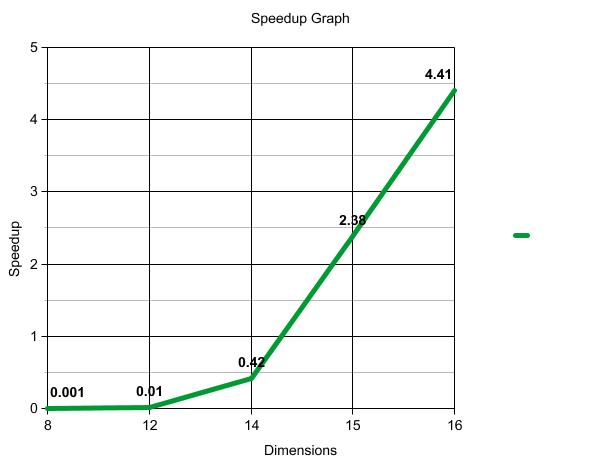
\includegraphics[width=\linewidth]{graph.jpg}
  \caption{The speedup graph}
\end{figure}

As can be seen there was a pretty linear speedup presented. The graph shows that as the iterations and size of the problem increased, the speedup also increased in a pseudo-exponential way at first before
moving more linearly upward.

\section{Conclusion}
This project was definitely a journey. Trying to wrestle through OpenMPI configurations and getting the code to work in parallel more efficiently proved to be an interesting challenge that really
stretched what I thought I knew about distributed execution environments. Overall I am a little disappointed by my results, but I think in the context of a large, more easily split project, things
may have seen a much better speedup. I plan to continue using OpenMPI on my local cluster to see if I can improve the overall runtime in the future.

\end{document}
